\documentclass[12pt]{article}

\usepackage[font=footnotesize]{caption}
\usepackage{float}
\usepackage{epsf}
\usepackage{epsfig}
\usepackage{subfigure}
% \usepackage{subfig}
\usepackage{latexsym}
%\usepackage{algorithm}
%\usepackage[noend]{algorithmic}
% \usepackage{color}
\usepackage{color, colortbl}
\usepackage{wrapfig}
\usepackage{topcapt}
\usepackage{multirow}
\usepackage{tabularx}
\usepackage{hyperref}
\usepackage{xcolor}
\usepackage{mdwlist}
\usepackage{pdfpages} 

%\usepackage{color}
\newcommand{\lc}[1]{\textcolor{blue}{#1}}


\usepackage{amsmath, amsfonts, amssymb}
\usepackage[hmargin=1in,vmargin=1.2in]{geometry}
\usepackage{url}
\usepackage{multirow}
\usepackage[ruled,noline,linesnumbered]{algorithm2e}
\usepackage[bottom]{footmisc}
\usepackage{afterpage}
%\usepackage[caption=false]{caption}
\usepackage{eurosym}
\usepackage{enumitem}
% \usepackage{soul}
\usepackage{fancyhdr}
\usepackage{dashrule}
% \usepackage[stable]{footmisc}
% \usepackage{placeins}
% \setitemize{noitemsep,topsep=0pt,parsep=0pt,partopsep=0pt}
% \usepackage[utf8]{inputenc}
\usepackage{gensymb}

\widowpenalty=1000
\clubpenalty=1000

\input{epsf}

\def\nas{{NASA\ }}
\def\nase{{NASA}}
\def\esa{{ESA\ }}
\def\esae{{ESA}}
\def\inst{{NASA Ames Research Center\ }}
\def\inste{{NASA Ames Research Center}}
\def\univ{{UPorto\ }}
\def\unive{{UPorto}}
\def\soc{{SOCIB\ }}
\def\soce{{SOCIB}}
\def\vig{{UVigo\ }}
\def\vige{{UVigo}}
\def\ldeo{{LDEO\ }}
\def\ldeoe{{LDEO}}
\def\ls{{LSTS\ }}
\def\lse{{LSTS}}
\def\sml{{SmallSat\ }}
\def\smle{{SmallSat}}
\def\mba{{MBARI\ }}
\def\mbae{{MBARI}}
\def\rpe{{REP}}
\def\rp{{REP\ }}
\def\org{{SIFT\ }}
\def\orge{{SIFT}}
\def\pro{{\textmd{METEOR\ }}}
\def\proe{{\textmd{METEOR}}}
\def\kck{{Keck Foundation\ }}
\def\kcke{{Keck Foundation}}


\newlength{\doublespacelength}
\setlength{\doublespacelength}{\baselineskip}
\addtolength{\doublespacelength}{0.5\baselineskip}
\newcommand{\doublespace}{\setlength{\baselineskip}{\doublespacelength}}

\newlength{\singlespacelength}
\setlength{\singlespacelength}{\baselineskip}
\newcommand{\singlespace}{\setlength{\baselineskip}{\singlespacelength}}


\newlength{\savedspacing}
\newcommand{\savespacing}{\setlength{\savedspacing}{\baselineskip}}
\newcommand{\restorespacing}{\setlength{\baselineskip}{\savedspacing}}

\setlength{\parskip}{0pt}
\setlength{\parsep}{0pt}
\setlength{\headsep}{0pt}
\setlength{\topskip}{0pt}
\setlength{\topmargin}{0pt}
\setlength{\topsep}{0pt}
\setlength{\partopsep}{0pt}

\newcommand{\kc}[1]{{\color{red}{#1}}}
\newcounter{quotenumber}

\newenvironment{numquote}{%
    \begin{enumerate}%
     \setcounter{enumi}{\value{quotenumber}}%
     \color{darkgray}
    \item \begin{quote}%
}{%
    \end{quote}%
    \setcounter{quotenumber}{\value{enumi}}
    \end{enumerate}%
}%

\makeatletter
\def\myitem{%
   \@ifnextchar[ \@myitem{\@noitemargtrue\@myitem[\@itemlabel]}}
\def\@myitem[#1]{\item[#1]\mbox{}}
\makeatother
\definecolor{Gray}{gray}{0.6}


\newcommand\blankpage{%
    \null
    \thispagestyle{empty}%
    \addtocounter{page}{-1}%
    \newpage}

\setcounter{secnumdepth}{0} 


% \usepackage{picins}

\fancyhead[L]{}% empty left
\fancyhead[R]{ % right
    
\includegraphics[width=1.5in,height=0.45in]{fig/sift.jpg}\hspace{+0.09cm}
\includegraphics[width=0.95in,height=0.45in]{fig/uporto.png}
\includegraphics[height=0.45in]{fig/vigo.png}
\includegraphics[height=0.45in]{fig/ldeo.jpg}
\includegraphics[height=0.5in]{fig/socib.jpg}
}
\pagestyle{fancy}


\begin{document}

\vspace*{1cm}
\begin{center}
  {\large \bf{\proe}: A Portable Robotic Observatory for Diagnosing Coastal Ocean Health for Human Well Being}\\
  % \today
\end{center}

\vspace*{0.5cm}


% Modelling is related to 2 major actions: data integration (in situ and
% remote) through data assimilation and enhancing forecasting skills.


\subsection{Summary}
`

Our oceans host enormous biodiversity, provide multiple ecosystem
services, sustain vibrant economies, and play a significant role in
climate regulation, but are threatened by human activity and climate
change.  We need a \textbf{sustained}, \textbf{persistent}, and
\textbf{affordable} data gathering and assimilating capability to help
us understand and monitor how key processes such as acidification,
hypoxia, toxic blooms, pollution and erosion (amongst others) are
impacting global ocean sustainability and stewardship.  In coastal
regions, this is especially important, because these areas mediate
most of the interactions between a significant percentage of the world
population and the oceans.

Urban population growth has exacerbated the pressures on the coastal
ecosystem.  For example, resultant toxic blooms and oxygen depletion
have had deleterious effects on fisheries and other critical resources
that coastal populations depend on, while also impacting human
health. Furthermore, extreme weather events induced by climate change
will only hasten the worsening of water quality in these areas because
of enhanced runoff, coastal erosion and storm surges. An integrative
sea management approach and the protection of natural capital and
marine ecosystem resources can only be achieved with the help of
coordinated observations from space, aerial, surface and underwater
robots guided by Artificial Intelligence (AI) while providing
continual and reliable oceanographic data.

Many large telescopes point toward the heavens, but no such
observational system exists for looking at and into our oceans.  Our
mission is to build a portable, robotic observatory for observing,
analyzing and managing the health of our endangered coastal waters
which can be rapidly deployed anywhere in the world
(Fig. \ref{fig:mega-cities}).

\subsection{The Idea}

\pro (A Portable Robotic Observatory for Coordinated Oceanographic
Observations) will be a modular system with bespoke approaches related
to water quality in the world's coastal zones with mega-cities. It
will integrate state-of-the-art hardware including a small satellite
(\smle's) constellation, in-situ air, surface and underwater vehicles
with software to control and visualize the information gathered. With
frequent revisit times over a region by a constellation of \smle's,
coupled with latest smart and adaptive AI techniques, robots can
provide opportune observations in near real-time.

% robotic technologies reduces
% deployment time to provide opportune solutions and consequently,
% leverages the latest techniques in AI, Robotics and software
% engineering.


% It
% will provide information for water quality measurements suitable for
% lay persons who can obtain and interpret near real-time (hours) data
% visualized at spatial and temporal scales to provide actionable
% information to deal with coastal pollution, erosion, toxic waters and
% sediment laden plumes.


\begin{figure}[H]
  \centering
  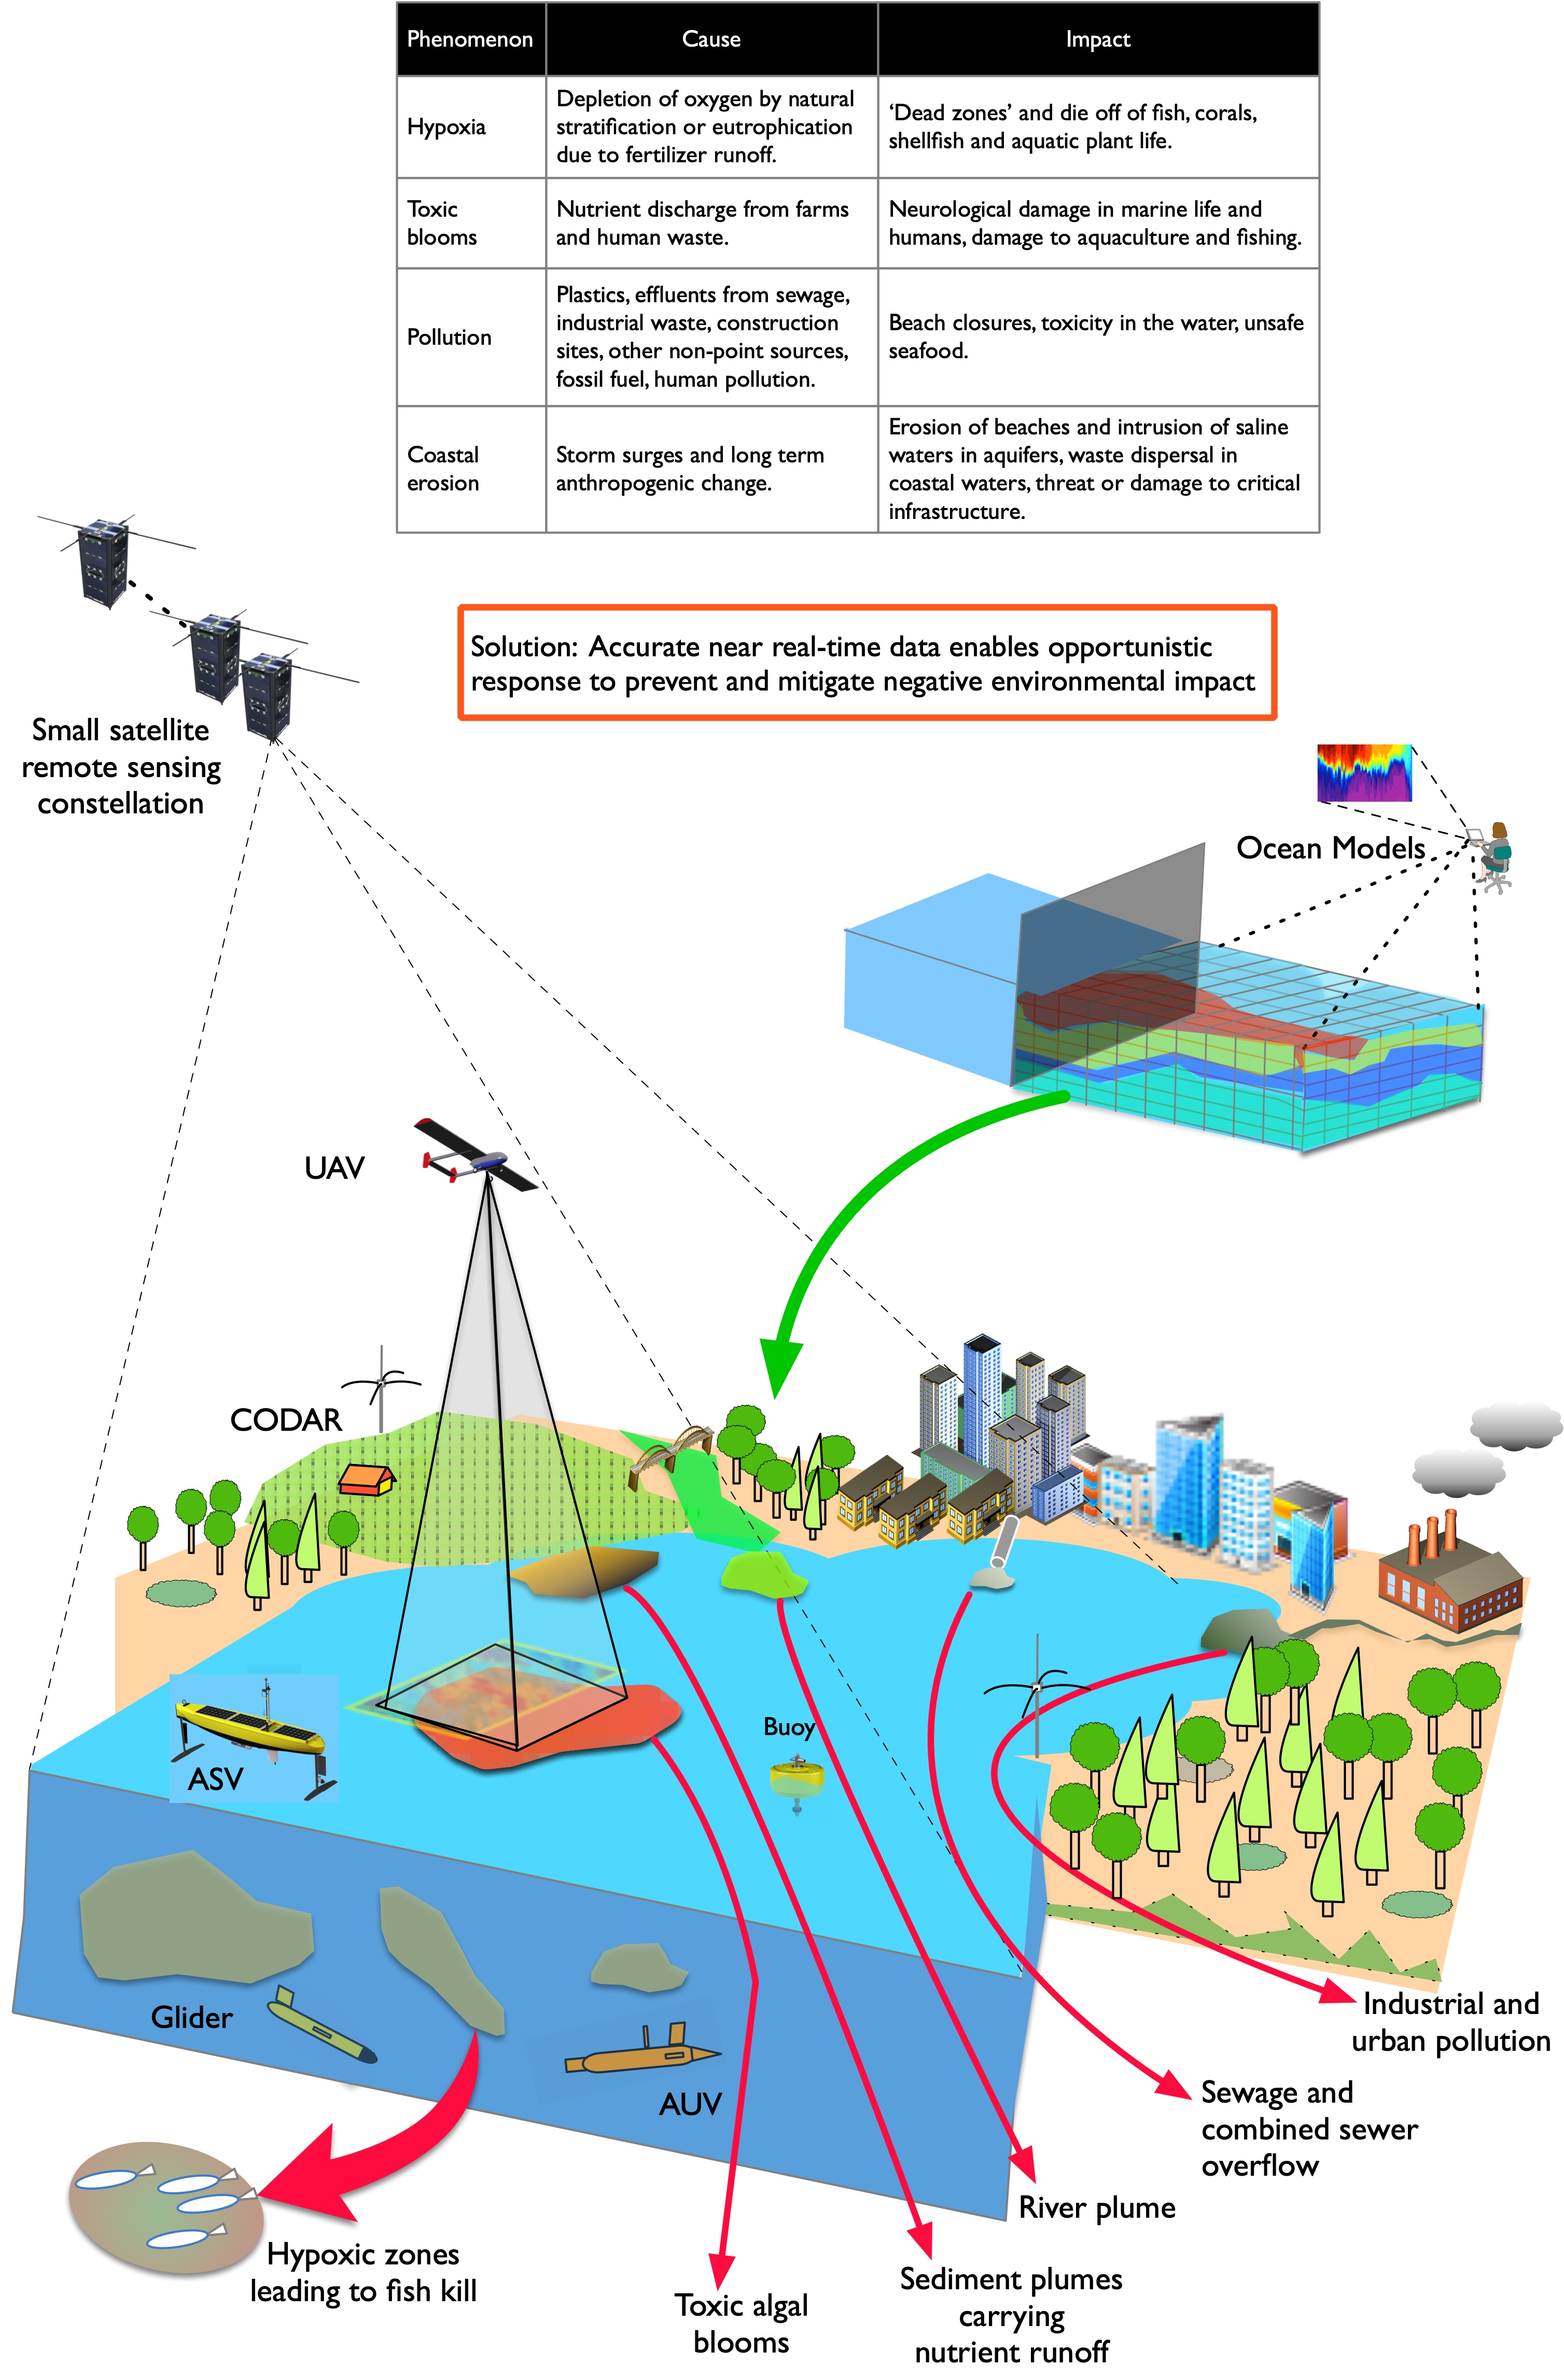
\includegraphics[scale=0.115]{fig/mega-cities-toxic-1.jpg}
  \caption{Coastal zones are impacted by natural and human-induced
    activities leading to oxygen depleted 'dead' zones, toxic algal
    blooms, pollution and coastal erosion. \pro will use an ensemble
    of small satellites, aerial, surface and underwater vehicles to
    observe the coastal ocean over sustained periods of time to
    provide real-time warning and situational awareness of impactful
    changes to human health, biodiversity and ecosystem services. Note
    the terms UAV: unmanned aerial vehicle, ASV: autonomous surface
    vehicle, AUV: autonomous underwater vehicle, CODAR: Coastal
    High-Frequency (HF) Radar.}
    \label{fig:mega-cities}
\end{figure}

Stakeholders across governments, industry, science, nonprofits and
citizenry will make use of layered views ranging from basic visuals to
the complex queries needed for effective management of resources and
increased scientific knowledge.  Ocean models will integrate the
information collected from multiple platforms robotic vehicles as well
as satellite remote sensing and to predict the evolution of
oceanographic conditions. This integration will provide a unified
picture of the surveyed water volume capturing the diversity of
phenomenon and connect that to natural ocean variability. The
model-data assimilated from robotic platforms will in turn allow us to
improve our understanding of the complex ocean flows and increase
predictive capability.
% Natural events such as storm surges, tsunamis and upwelled waters
% impact such mega-city coastal communities in addition. Turbulence in
% the upper water-column with potential injection of nutrients, either
% from the benthic or open ocean waters, can often result in sudden
% outgrowth of harmful algal blooms, or stirring up human-induced
% pollution in such coastal areas.

% In both human and nature induced events, the resulting mix can make it
% unsafe for any form of human activity often with no obvious and
% expected visible sign of near and present danger to local communities.
% However, the consequences can reverberate with mass scale die-off of
% marine life, poisoned shellfish and coastal wildlife and as well as
% causing neurological damage or fatalities to the human population on
% consuming seafood or using beaches for recreation.

% Current forms of monitoring are based on sensors (if present) spaced
% well apart, periodic human-made measurements that can be impacted by
% harsh weather and which typically sub-sample such dynamic coastal
% environments.

% \pro will integrate state-of-the-art hardware including a small
% satellite (\smle) constellation, in-situ air, surface and underwater
% vehicles with software to control and visualize information derived
% from these assets.  The use of \smle's and smart robotic technologies
% reduces deployment time to provide opportune solutions and
% consequently leverages the latest techniques in AI, Robotics and
% software engineering. Coordinated perspectives across different
% synoptic spatial and temporal scales in turn will provide a
% hyper-realistic situational assessment to stakeholders including those
% who drive policy making for human health.

% In the report, “Global Marine Trends 2030”, Lloyds Register predicts
% that by 2030, the coastal ocean will be “almost unrecognizable”. As we
% enter the United Nations “Decade of the Ocean”, \pro will broaden and
% deepen knowledge that will aid and augment global ocean sustainability
% and stewardship, and the management of our Urban Seas.

\subsection{Why now?}

With the onset of a climate crisis, the oceans are changing rapidly in
ways we do not understand. In the report, ``Global Marine Trends
2030'', Lloyds Register predicts that by 2030, the coastal ocean will
be ``almost unrecognizable''. There is an urgent need to develop and
deploy new smart observational methods to provide information at
scales that matter to the 600 million people living along the coast
within 10 meters of the sea level.  Predicting change and providing
early warning of hazardous events is essential for the well-being of
an increasingly vulnerable coastal ecosystem. It is also in line with
the goals of the 2021-2030 UN Decade of Ocean Science for Sustainable
Development.

% The oceans cover more than 70\% of the earth's surface. The base of
% the human food-chain starts with tiny phytoplankton which generate the
% oxygen for every other breath we take.  With the onset of a climate
% crisis, the oceans are changing rapidly in ways we do not
% understand. There is an urgent need to develop and deploy new smart
% observational methods to provide information at scales that matter to
% the 600 million people living along the coast within 10 meters of the
% sea level.  Predicting change and providing early warning of hazardous
% events, including poor water quality, tainted fish stocks and
% intensifying coastal erosion, is essential for the well-being of an
% increasingly vulnerable coastal ecosystem. It is also in line with the
% goals of the 2021-2030 UN Decade of Ocean Science for Sustainable
% Development.

% By leveraging rapid advances in technology, \pro will field an
% innovative system of small satellites and robust autonomous in-situ
% platforms for obtaining unprecedented views of coastal oceans and
% atmospheric and land interfaces. It will aid in the understanding and
% monitoring of coastal waters so that they can be explored and utilized
% in a sustainable and informed manner.

% \pro will leap-frog the traditional incremental and siloed methods in
% ocean observation by leveraging modern computational methods in data
% science, autonomous robotics and smart sensors. The density and
% diversity of observations will change by an order of magnitude, the
% temporal scales of coastal observations will change from weeks (for
% traditional shipboard sampling) or days (for existing satellite data)
% to hours and minutes with the provision of real-time information.


\vspace*{0.1cm}
\subsection{What is the novelty?}

\pro is different from traditional methods for observing the coastal
ocean, which are inefficient, not cost-effective, too sparse in space,
too sporadic in time or too localized. There is poor integration and
assimilation of multiple data sources especially between those made
in-situ and those made by satellites to produce actionable knowledge.
% for 21\textsuperscript{st} century decision making.

\pro leap-frogs current methods by delivering predictive modeling,
learning and analytical capabilities, which are supported by AI and
visualization techniques that are non-existent in other interventions.
With \proe, the density and diversity of observations will change by an
order of magnitude, the temporal scales of coastal observations will
change from weeks (for traditional shipboard sampling) or days (for
existing satellite data) to \emph{hours and minutes} with the
provision of real-time information. Techniques in AI will adapt the
information depending on the kind of user, from well-informed
scientists, to the lay person curious about how beach conditions might
impact her leisure. 

% Using AI will adapt the kind of information depending on the kind of
% user. 

In the process of providing actionable knowledge, \pro will enable new
modes of management and new understanding about coastal ocean
processes in ways simply not possible before. \pro will allow citizens
to develop critical understanding of the rapid change taking place in
their Urban Seas and to ‘connect the dots’ between human activity and
the effect on the environment around them. Citizen scientists will be
engaged in generating new observations and be able to derive new
knowledge about how ocean processes work. Scientists will be able to
pose (and answer) new questions that could not have been asked
before. And policy makers will have the tools to make informed
decisions in time scales that matter, while developing truly
integrative policies on ocean sustainability and
stewardship. % \pro will serve as a replicable blueprint for Ocean
% observation in targeting integration, synthesis, cost-effectiveness
% and scalability.

% While some coastal ocean observatories use a limited number of robotic
% assets or remote sensing data, \pro is unique in the range and
% diversity of how these sensors are deployed, how data is integrated
% and synthesized, and how citizen engagement is used to improve the
% value of the output.  Additionally \pro provides an integrative
% open-source framework to connect robots, services and users in a
% seamless manner that is both scalable and replicable, providing a
% blueprint for other initiatives worldwide. It leap-frogs current
% methods by delivering 21st century predictive modeling, learning and
% analytical capabilities, which are supported by AI and visualization
% techniques that are non-existent in other interventions.

\subsection{Milestones and Deliverables}


\begin{figure}[!t]
  \centering
  \subfigure[]{\label{fig:insitu}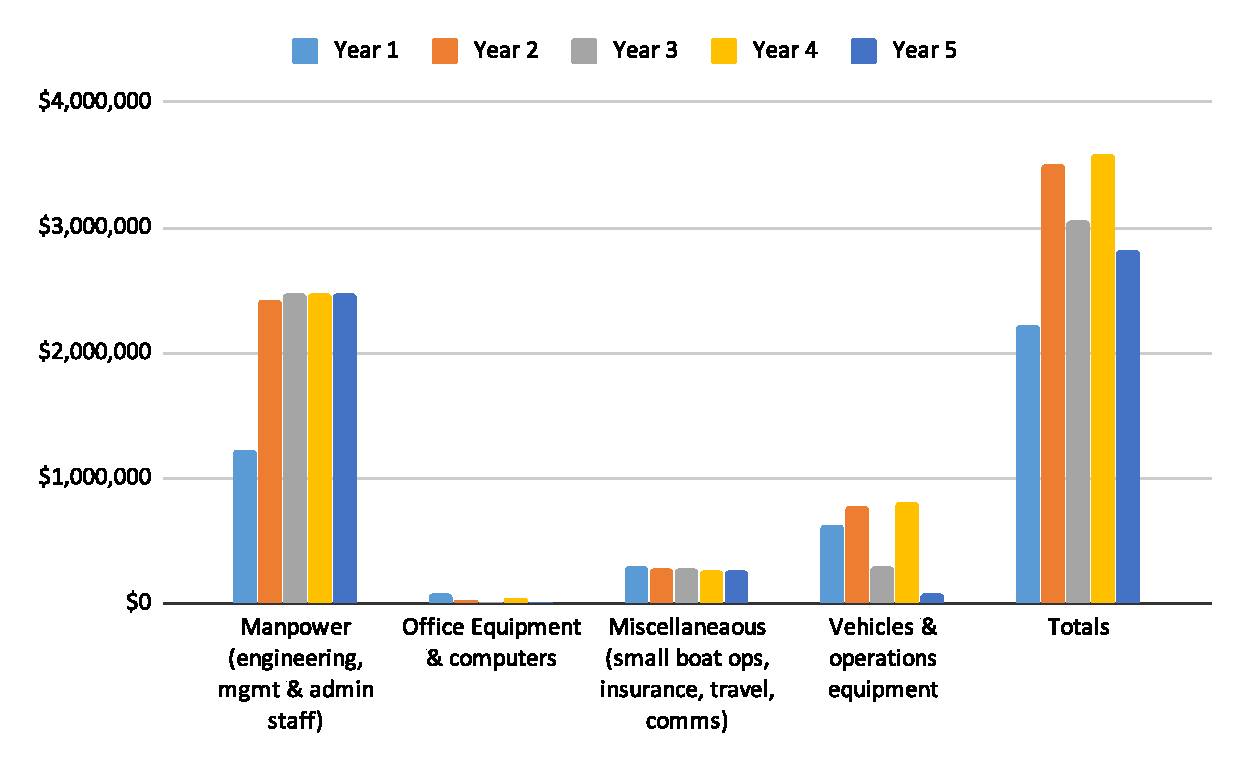
\includegraphics[scale=0.35]{fig/insitu.pdf}}
  \subfigure[]{\label{fig:sats}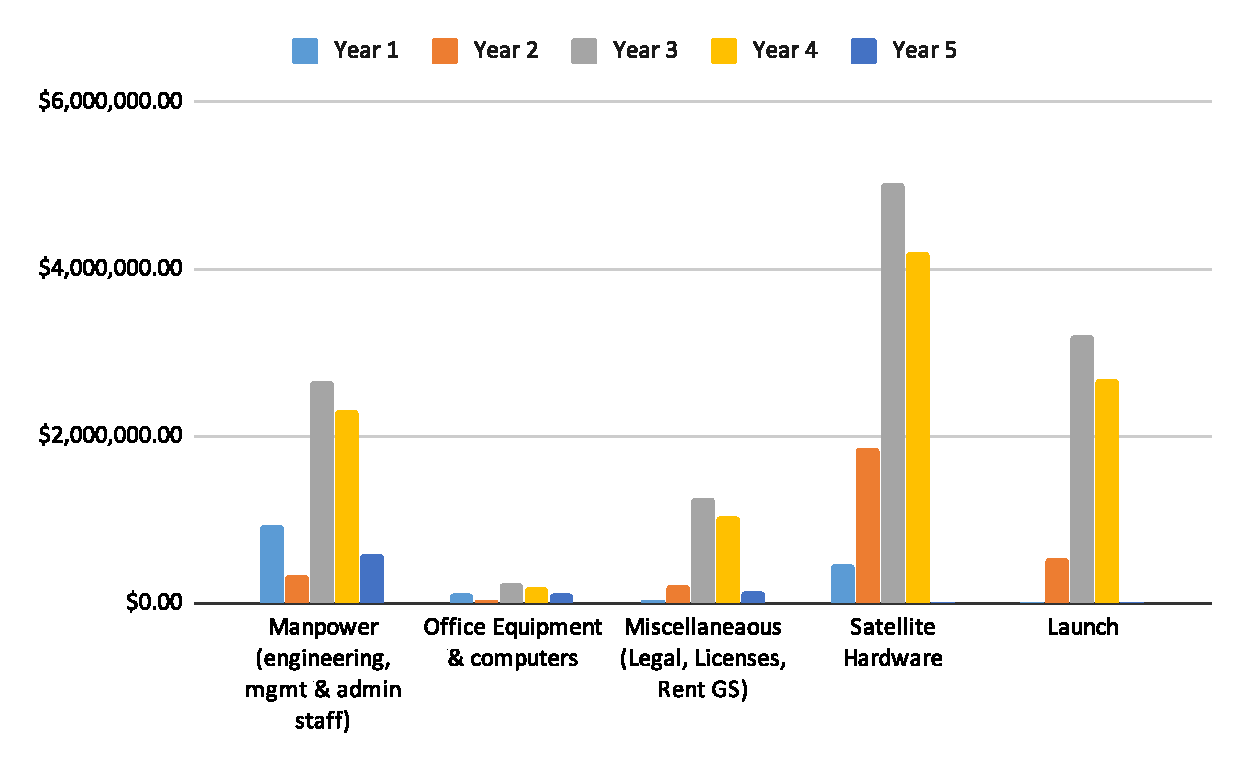
\includegraphics[scale=0.35]{fig/sats.pdf}}
  \caption{Costs and distribution for \ref{fig:insitu} in-situ robotic
    assets, control and visualization software and \ref{fig:sats}
    \smle's over a 5 year project term.}
  \label{fig:costs}
  \vspace{-0.5cm}
\end{figure}


\begin{itemize}[noitemsep,topsep=0pt,parsep=0pt,partopsep=0pt]

\item Architectural design of the system with a focus on software
  integration, building hardware and design and testing of Machine
  Learning systems for ocean model prediction (Year \textbf{1})

\item Use of existing remote sensing data products (e.g. ESA and NASA
  data products), integration of ocean models and building of AI-based
  adaptive control systems for aerial, surface and underwater
  vehicles.  (Years \textbf{1--2})

\item Incremental at-sea testing of adaptations of robotic vehicles
  and integration of control with ocean model predictions (Years
  \textbf{2--3}) 

  % \piccaption[]{Hello Text}
  % \parpic(3in,2.5in)[r]{\label{fig:insitu}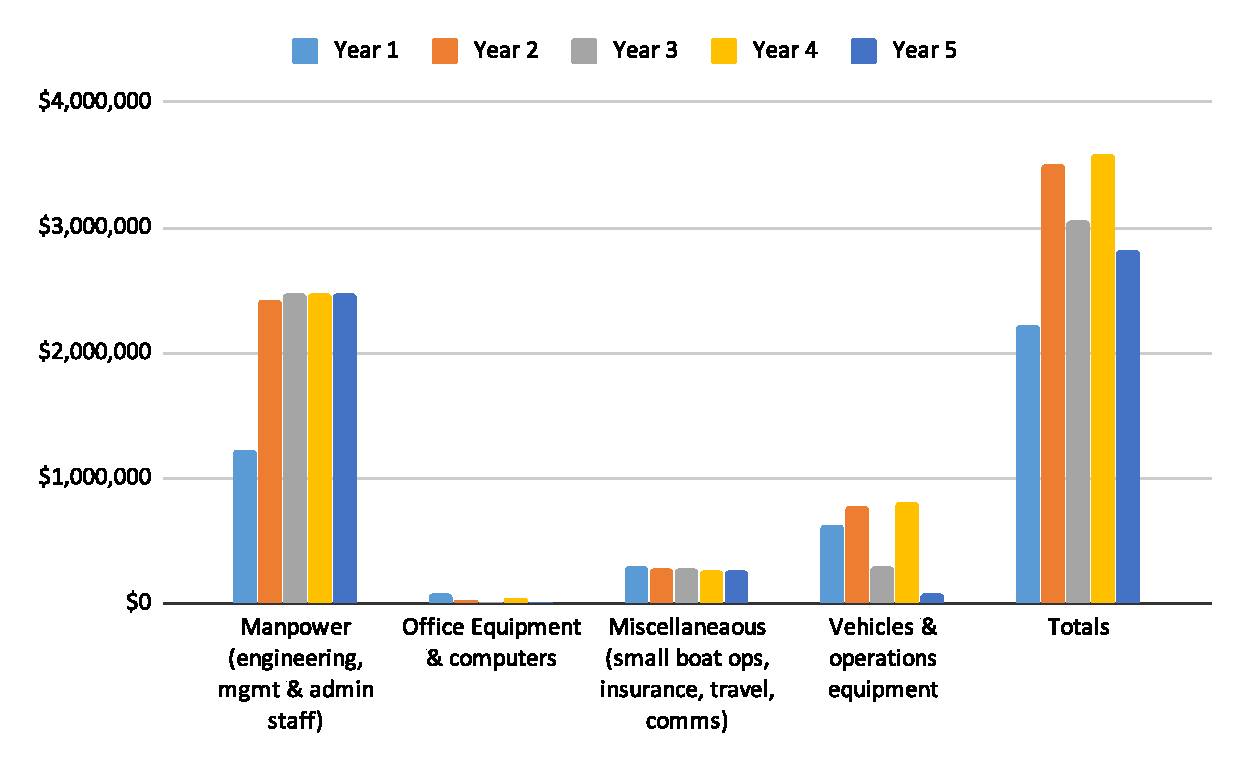
\includegraphics[scale=0.4]{fig/insitu.pdf}}
  
\item Demonstration of the integrative software system using existing
  aerial, surface and underwater vehicles from the Univ. of Porto and
  targeting a single extensive use-case (e.g. from aquaculture, oil \&
  gas, others) to monetize this effort (Year \textbf{3})

\item Upscope demonstration to include larger data sources for
  physical ocean properties, including from buoys and synthetic data
  sources (e.g. surf forecasts). If \sml budget permits, begin design
  and build of satellite elements including payload elements (Years
  \textbf{3--4})

\item \sml launch and operation begins. Validation of satellite
  payloads and calibration of sensor performance (Years \textbf{4--5})

\item Pursue European Union and other large funding schemes to fund a
  larger constellation of \smle's to demonstrate the full capability
  in a coastal meso-scale ($\sim 50$ Km\textsuperscript{2}) ecosystem
  (Years \textbf{3--5})

\end{itemize}

\begin{wrapfigure}{r}{0.45\textwidth}
  % \vspace{-1cm}
  \centering
  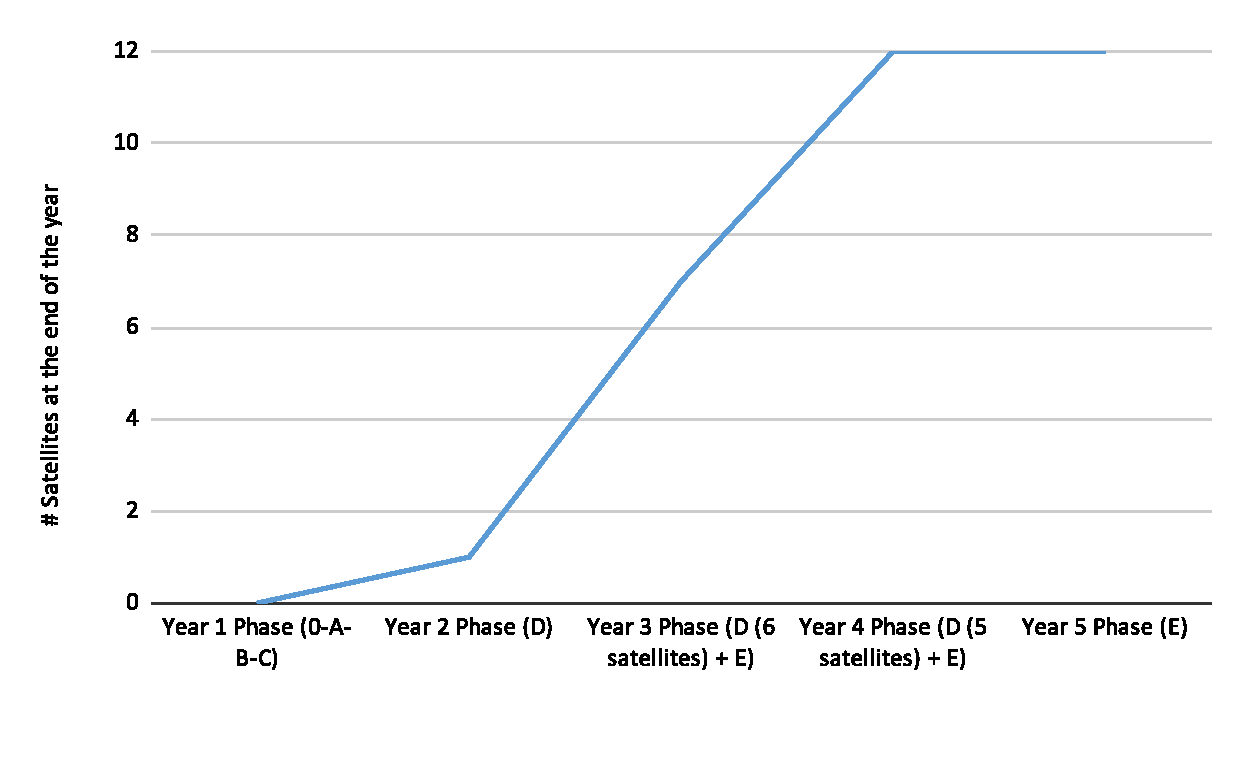
\includegraphics[scale=0.35]{fig/sat-progression.pdf}
  \caption{Progression of deployment for 12 \smle's over a period of 5
    years.}
  \label{fig:sat-prog}
  % \vspace{-0.5cm}
\end{wrapfigure}

\newpage
Fig. \ref{fig:costs} shows costs associated with the project broken
down for in-situ robotic assets and for \smle's, to provide a clear
picture of the distributions of proposed expenses. Should the \sml
part of the project be simultaneously executed with the development of
software and hardware for in-situ assets, the two figures would then
be merged. The incremental deployment of the \smle's is shown in
Fig. \ref{fig:sat-prog}. 

% \parbox[t]{\dimexpr\textwidth-\leftmargin}{%
%       \vspace{-2.5mm}
%       \begin{wrapfigure}[10]{r}{0.5\textwidth}
%         \centering
%         \vspace{-\baselineskip}
%         \subfigure[]{\label{fig:insitu}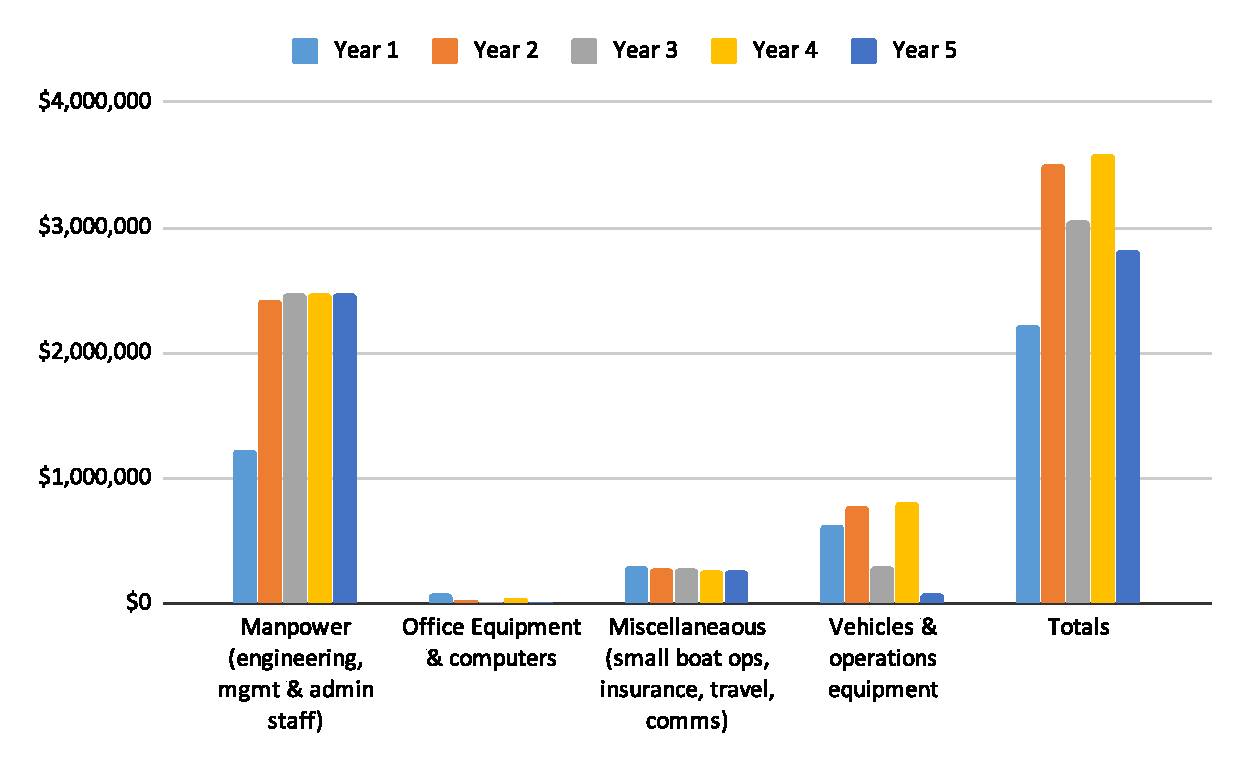
\includegraphics[width=.75\linewidth]{fig/insitu.pdf}}
%         \subfigure[]{\label{fig:sats}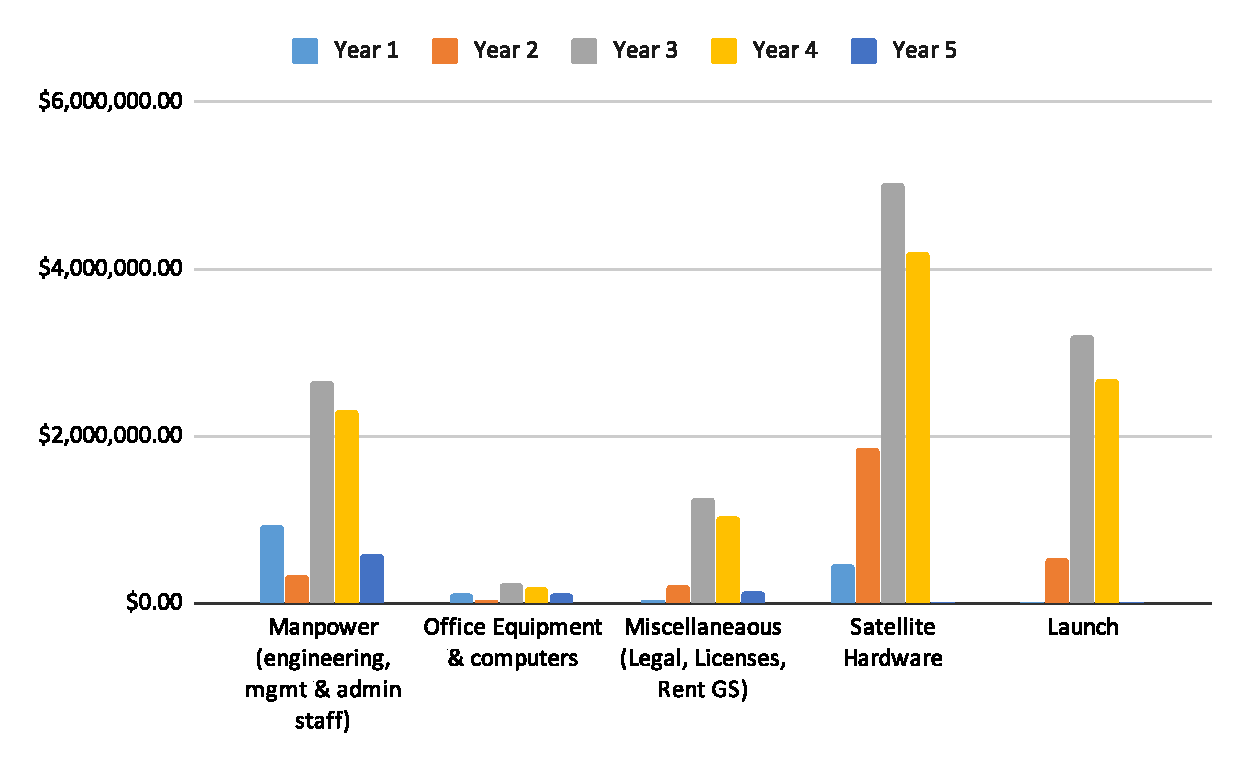
\includegraphics[width=.75\linewidth]{fig/sats.pdf}}
%         \caption{Costs and distribution for \ref{fig:insitu} assets and
%           software and \ref{fig:sats} \smle's over a 5 year project term.}
%       \end{wrapfigure}
%     }

\subsection{Resources Needed}

The \pro team comes ready with the aerial, surface and underwater
vehicle platforms, together with the extensive suite of communication
software to provide coordinated observations in the coastal ocean. We
will integrate custom sensors keyed towards important ocean variables
integrated into a 'train' of \sml platforms.  Such a system working
synchronously with in-situ robots will provide a clear consistent set
of data products. This data will be integrated to provide actionable
information to policymakers on the ground, as also society in general.

We estimate the total project cost to be $\sim \$63.5$ Million over a
period of 5 years. As milestones are met in the first two years, and
the integrated software can be demonstrated on targeted use-cases,
\pro is likely to attract funding from public and private
sources. Consequently, the project can also be funded in incremental
steps:

\begin{itemize}[noitemsep,topsep=0pt,parsep=0pt,partopsep=0pt]

\item an initial focus on the software build, integration and test
  with available robotic vehicles in small scale demonstrations $\sim
  \$5$--$\$10$ Million for years 1 \& 2.

\item acquisition of robotic vehicles, buoys, floats and a range of
  sensors as payloads for these in-situ vehicles, their integration,
  deployment and demonstration at increasingly larger spatial and
  temporal scales for $\sim \$20$--$\$30$ Million in years 2 \& 3.

\item acquisition of funds for a suitable at-scale design, build,
  test, launch and operation of a \sml constellation with a range of
  scientific payloads for biological and physical oceanographic
  measurements for $\sim \$25$ Million in years 4 \& 5.

\end{itemize}  

Incremental build and evaluation of this concept can allow us to
attract a wide range of public and private sponsors in the US and
Europe.  Equally, we will consistently work with our collaborators in
the Portuguese government to leverage expensive ship time for testing,
and other potential in-kind contributions from Portuguese and Spanish
resources.

For long-term operation and viability of this system, multiple
outcomes can be envisioned. First, with the experience garnered in
testing and fielding the system, a commercial spin-off of all or parts
of the technology could be very possible. If parts of the technology
could be monetized and spun off to other companies, \pro can then hold
the IP while continuing to work on research outcomes after the 5 year
term. Second, the project can itself look for contracts from
mega-cities and governments or their agencies to provide a
software-as-a-service model and be able to subsist as a not-for-profit
enterprise with unique expertise. Should other private or public
funding sources be available, those would also be carefully evaluated
at this time.


\subsection{Governance}

The governing board of \pro will consist of prominent strategic
advisors from the US and Europe including stakeholders and funders. In
addition, the project principals will be aided and advised by a
scientific advisory board consisting of technologists, ocean going
scientists, ecologists and policy makers from the US, Europe and
targeted coastal states.

\subsection{The Team}

\proe’s inter-disciplinary team of seasoned researchers (see bio's
below) from the universities of Columbia/US, Porto/Portugal and
Vigo/Spain have worked in all the major oceans, fielded tens of robots
at sea simultaneously, designed/built/flown and operated multiple
\smle's and complex systems in the deep sea and deep space.

\newpage
\section{Brief Bios of the Principals}

\parbox{6.5in}{
\begin{wrapfigure}{r}{0.45\textwidth}
  \centering
  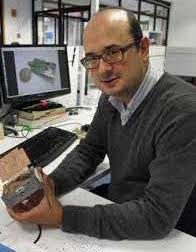
\includegraphics[width=.75\linewidth]{fig/FAguado.jpg}
\end{wrapfigure}
\textbf{Fernando Aguado} is an Associate Professor at the University
of Vigo. He was the principal investigator (PI) of the Xatcobeo
cubesat, the first Galician satellite and the first Spanish
cubesat. He was also the PI of HUMSAT-D and sector B of Serpens (both
developed within the Basic Space Technology Initiative of UN with the
support of ESA) and the LUME-1 \smle. He has coordinated the design,
manufacturing and integration of various Cubesats for maritime and
airplane tracking applications as well as for inter-vehicle
communications. 
\\
\textbf{email: }\emph{faguado@tsc.uvigo.es} \\
\textbf{Web: }\url{https://bit.ly/3avJlwX}\\
}

\parbox{6.5in}{
\begin{wrapfigure}{r}{0.45\textwidth}
  \centering
  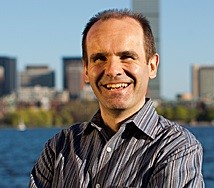
\includegraphics[width=.75\linewidth]{fig/Pierre.jpg}
\end{wrapfigure}
\textbf{Pierre Lermusiaux} is Professor of Mechanical Engineering and
Ocean Science and Engineering at MIT, and, since July 2018, Associate
Department Head for Research and Operations in Mechanical
Engineering. He has made outstanding contributions in data
assimilation, as well as in ocean modeling and uncertainty
predictions. His research thrusts include understanding and modeling
complex physical and interdisciplinary oceanic dynamics and processes
while utilizing new mathematical models and computational methods for
ocean predictions and dynamical diagnostics for data assimilation
and data-model comparisons.
\\
\textbf{email: }\emph{pierrel@mit.edu}\\
\textbf{Web:}\url{http://web.mit.edu/pierrel/www/} 
}

\parbox{6.5in}{
\begin{wrapfigure}{r}{0.45\textwidth}
  \centering
  \includegraphics[width=.75\linewidth]{fig/Krajan.jpg}
\end{wrapfigure}
\textbf{Kanna Rajan}\footnotemark\footnotetext{Principal point of
  contact} is a Fellow at SIFT LLC and holds a visiting faculty
appointment at the \univ in autonomous systems. He spent 10 years at
\inst where his software was responsible for the command/control of
the 1999 New Millennium Deep Space 1, 65 Million miles from Earth and
the 2003 Mars Exploration Rovers mission on the Red Planet. In 2005 he
moved to \mba and built the only AI group in marine robotics. His
field work and publications have been in highly ranked peer-reviewed
publications including \emph{Science}, Intnl. Journal of Robotics
Research, the AI Journal and Journal of Field Robotics. He has
participated in scientific oceanographic cruises in the Pacific and
Atlantic.
\\
\textbf{email: }\emph{Kanna.Rajan@sift.net}\\
\textbf{Web:}\url{https://www.sift.net/staff/kanna-rajan} 
}

\vspace*{0.5cm}
\parbox{6.5in}{
\begin{wrapfigure}{r}{0.45\textwidth}
  \centering
  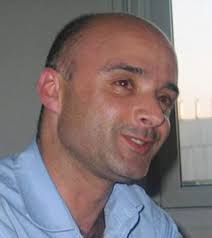
\includegraphics[width=.75\linewidth]{fig/JBS.jpg}
\end{wrapfigure}
\textbf{Jo\~ao Sousa} is a Professor at the Faculty of Engineering,
Univ. of Porto, Portugal and the head of the Underwater Systems and
Technology Laboratory (\lse). The lab has pioneered the design,
construction and deployment of networked underwater, surface and air
vehicles for applications in ocean sciences and defense and is at the
vanguard of operations of coordinated aerial, surface and underwater
vehicles. The lab designed the award-winning Light Autonomous
Underwater Vehicle and the \ls open source software for networked
vehicle systems, and has been key in organizing large scale
experiments, including the annual Rapid Environmental Picture (\rpe)
organized jointly with the Portuguese Navy since 2010. He has
participated and led numerous engineering and scientific oceanographic
cruises.
\\
\textbf{email: }\emph{jtasso@fe.up.pt}\\
\textbf{Web: }\url{https://bit.ly/2J6cKCc}}
% {https://lsts.pt/member/jo%C3%A3o-sousa}

% \vspace*{0.5cm}
\parbox{6.5in}{
\begin{wrapfigure}{r}{0.45\textwidth}
 \centering
  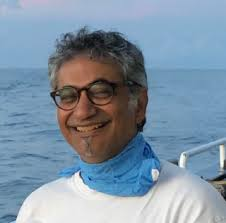
\includegraphics[width=.75\linewidth]{fig/ASub.jpg}
\end{wrapfigure}

\textbf{Ajit Subramaniam} is a Lamont Research Professor at the
Lamont-Doherty Earth Observatory (\ldeoe) of Columbia University, New
York.  He is an oceanographer who uses knowledge of remote sensing,
ocean optics, phytoplankton physiology, biological and physical
oceanography and geographical information systems to better understand
how the marine ecosystem functions and can be managed.  He has worked
for National Oceanic and Atmospheric Administration (NOAA), and held
appointments at the Univ. of Maryland and the Univ. of Southern
California prior to moving \ldeo in 2004. He has served as the Program
Director for the Marine Microbiology Initiative at the Gordon and
Betty Moore Foundation and a program manager in the Biological
Oceanography Program at the U.S. National Science Foundation (NSF). He
has participated in oceanographic cruises in all parts of the world.
\\
\textbf{email: }\emph{ajit@ldeo.columbia.edu} \\
\textbf{Web: }\url{https://www.ldeo.columbia.edu/~ajit/}
}

\vspace*{0.5cm}
\parbox{6.5in}{
\begin{wrapfigure}{r}{0.45\textwidth}
 \centering
  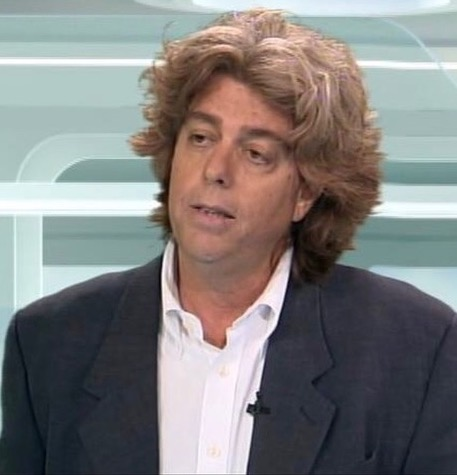
\includegraphics[width=.75\linewidth]{fig/JTintore.jpeg}
\end{wrapfigure}

\textbf{Joaqu\'{i}n Tintor\'{e}} is Professor of Physical Oceanography
and Director of the Spanish Large-Scale Marine Infrastructure SOCIB
(Balearic Islands Coastal Ocean Observing and Forecasting System) that
he proposed and designed in 2006. His present scientific interest is
in understanding ocean state and variability, from episodic events to
climate variability from the coast to the open ocean while
implementing new multi-platform and integrated ocean observing and
forecasting systems.
\\
\textbf{email: }\emph{jtintore@socib.es} \\
\textbf{Web:
}\url{http://www.socib.eu/?seccion=textes&id_textotextes=director} }


\end{document}

